\begin{figure}[t]\centering
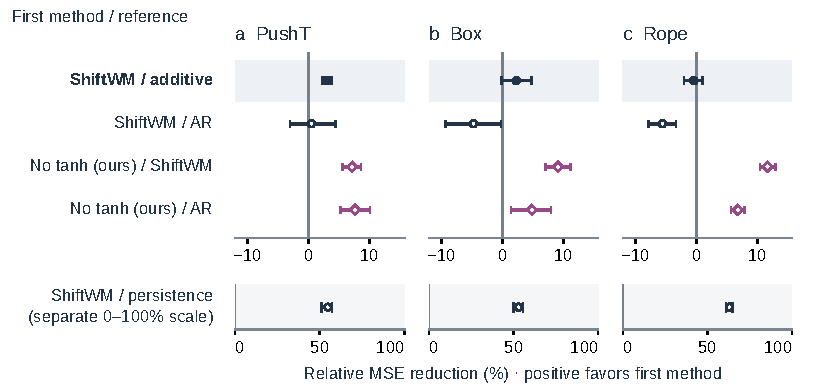
\includegraphics[width=\linewidth]{generated/iws_reserved_evidence/reserved_comparisons.pdf}
\caption{\textbf{Reserved IWS feature forecasts.} Points and bars show $H=60$ relative standardized-MSE reductions, $100(b-m)/b$, and paired 95\% seed--trajectory intervals (10,000 draws, seed 173). Each row names method $m$ and reference $b$; positive favors $m$. The filled first row---bounded ShiftWM (ours) versus additive anchoring---is primary. Hollow circles mark other ShiftWM contrasts; diamonds mark our post-development no-$\tanh$ ablation. The bottom persistence strip uses a separate, labeled 0--100\% scale. Estimates equally weight trajectories and learned seeds (three seeds; 200 handles from ten trajectories per task). All 36 predictors use the same post-access row-wise GRU revision after an input-only audit; weights, examples, metrics and tolerances remain fixed. Tables~\ref{tab:iws-reserved-scores} and~\ref{tab:iws-reserved-standardized-mse-contrasts} give all metric means and signed MSE effects, including the equal-task macro.}
\label{fig:iws-reserved-comparisons}\end{figure}
